\documentclass[11pt]{article}
\usepackage{amsmath, amssymb, amsthm}
\usepackage[retainorgcmds]{IEEEtrantools}

\usepackage[pdftex]{graphicx}
\usepackage{tikz}
\usetikzlibrary{intersections}

\usepackage{marginnote}
\usepackage{endnotes}

\usepackage{fancyhdr}

%Listings stuff
\usepackage{listings}
\usepackage{lstautogobble}
\usepackage{color}

\definecolor{gray}{rgb}{0.5,0.5,0.5}
\lstset{
basicstyle={\small\ttfamily},
tabsize=3,
numbers=left,
numbersep=5pt,
numberstyle=\tiny\color{gray},
stepnumber=2,
breaklines=true
}

%Properly formatted differential 'd'
\newcommand{\ud}{\, \mathrm{d}}

%Format stuff
\pagestyle{fancy}
\headheight 35pt

%Header info
\chead{\Large \textbf{Heaps}}
\lhead{}
\rhead{}

\begin{document}
\section{Properties}
	A heap is a generic container for objects with comparable keys. Inserting, deleting, and extracting the minimum or maximum (depending on the heap implementation) are all $O(\log n)$ operations, and heapifying an entire list is an $O(n)$ operation.
	
	\subparagraph{Heapsort} Heapsort \marginnote{Heapsort?}is a very simple $O(n\log n)$ sort that heapifies a list to be sorted, then extracts the minimum from the top of the heap until the heap is empty.
	
\section{Implementation}
	\marginnote{Efficient representation?}Conceptually, a binary heap is a rooted binary tree that is as complete as possible. In a min-heap, at every node \verb|x|, \verb|key[x]|$\leq$ all child keys.
	
	\begin{center}
	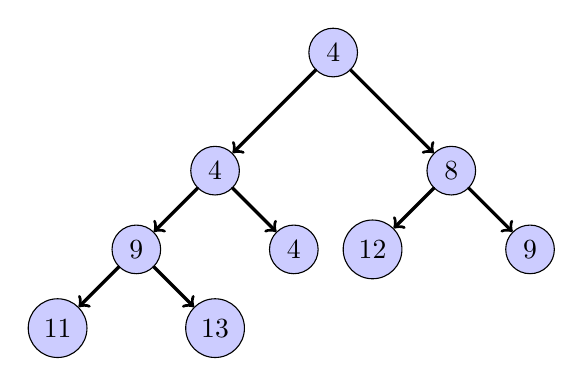
\begin{tikzpicture}
		[scale=.5,line cap=round,
		%Styles
		axes/.style=,
		important line/.style={very thick},
		information text/.style={rounded corners,fill=red!10,inner sep=1ex},
		dot/.style={circle,inner sep=1pt,fill,label={#1},name=#1},	
		main node/.style={circle,fill=blue!20,draw}		
		]
		
		%Colors
		\colorlet{anglecolor}{green!50!black}	%angle arcs/lines
		
		\node[main node] (1) at (0,0) {4};
		\node[main node] (2) at (-3,-3) {4};
		\node[main node] (3) at (3, -3) {8};
		\node[main node] (4) at (-5, -5) {9};
		\node[main node] (5) at (-1, -5) {4};
		\node[main node] (6) at (1, -5) {12};
		\node[main node] (7) at (5, -5) {9};
		\node[main node] (8) at (-7, -7) {11};
		\node[main node] (9) at (-3, -7) {13};
		
		\path[->, very thick]
			(1)	edge (2)
				edge (3)
			(2)	edge (4)
				edge (5)
			(3)	edge (6)
				edge (7)
			(4) edge (8)
				edge (9);
	\end{tikzpicture}
	\end{center}
	A binary heap can be intuitively represented by an array. The above heap would be represented as \verb|[4 4 8 9 4 12 9 11 13]|. The relationship between array elements is as follows for a 0-based array.
	\begin{itemize}
		\item \marginnote{Parent and child indexing?}\verb|parent(i)| = $(i-1)/2$
		\item \verb|children(i)| = ($2i + 1$, $2i + 2$)
	\end{itemize}
	
	\subsection{Command Implementation}
		\marginnote{Bubbling?}Every basic heap manipulation depends on two basic algorithms: bubble-up and bubble-down. Apart from that, it is possible to insert an element, extract the root, delete an element, and heapify a collection.
		
		\subparagraph{Bubble Up} To bubble up, check if the heap property is violated by comparing an element with its parent. If it is, swap the two and repeat with the same element in the new position.
		
		\subparagraph{Bubble Down} Compare the element with its children, and if the heap property is violated, swap the element with the smaller child, and repeat.
		
		\subparagraph{Insert} Append the new element $k$ to the end of the array, and bubble up.
		
		\subparagraph{Extract} Remove the root, move the last leaf node to the root, and bubble down.
		
		\subparagraph{Delete} Remove the element, swap the last leaf node to its position, and bubble up or down as necessary.
		
		\subparagraph{Heapify} Read data into an array, and starting from the lowest, rightmost parent node, bubble down.

%	\begin{center}
%	\begin{tikzpicture}
%		[scale=3,line cap=round,
%		%Styles
%		axes/.style=,
%		important line/.style={very thick},
%		information text/.style={rounded corners,fill=red!10,inner sep=1ex},
%		dot/.style={circle,inner sep=1pt,fill,label={#1},name=#1}			
%		]
%		
%		%Colors
%		\colorlet{anglecolor}{green!50!black}	%angle arcs/lines
%		
%		%The graphic
%	\end{tikzpicture}
%	\end{center}

%	\begin{figure}[htb]
%		\centering
%		\includegraphics[width=0.8\textwidth]{filename.eps}
%		\caption{Caption.}
%		\label{fig:figure}
%	\end{figure}

%		\def\enotesize{\normalsize}
%		\theendnotes
\end{document}